
\documentclass[12pt]{extarticle}
%Some packages I commonly use.
\usepackage[english]{babel}
\usepackage{framed}
\usepackage[normalem]{ulem}
\usepackage{amsmath}
\usepackage{amsthm}
\usepackage{amssymb}
\usepackage{amsfonts}
\usepackage{enumerate}
\usepackage[top=1 in,bottom=1in, left=1 in, right=1 in]{geometry}
\usepackage{graphicx}
\usepackage[utf8]{inputenc} % Required for inputting international characters
\usepackage[T1]{fontenc} % Output font encoding for international characters
\usepackage{mathpazo} % Palatino font
\usepackage{xfrac}% http://ctan.org/pkg/xfrac

%A bunch of definitions that make my life easier
\newcommand{\matlab}{{\sc Matlab} }
\newcommand{\cvec}[1]{{\mathbf #1}}
\newcommand{\rvec}[1]{\vec{\mathbf #1}}
\newcommand{\ihat}{\hat{\textbf{\i}}}
\newcommand{\jhat}{\hat{\textbf{\j}}}
\newcommand{\khat}{\hat{\textbf{k}}}
\newcommand{\minor}{{\rm minor}}
\newcommand{\trace}{{\rm trace}}
\newcommand{\spn}{{\rm Span}}
\newcommand{\rem}{{\rm rem}}
\newcommand{\ran}{{\rm range}}
\newcommand{\range}{{\rm range}}
\newcommand{\mdiv}{{\rm div}}
\newcommand{\proj}{{\rm proj}}
\newcommand{\R}{\mathbb{R}}
\newcommand{\N}{\mathbb{N}}
\newcommand{\Q}{\mathbb{Q}}
\newcommand{\Z}{\mathbb{Z}}
\newcommand{\<}{\langle}
\newcommand\tab[1][1cm]{\hspace*{#1}}
\newcommand{\attn}[1]{\textbf{#1}}
\newcommand{\bproof}{\bigskip {\bf Proof. }}
\newcommand{\eproof}{\hfill\qedsymbol}
\newcommand{\Disp}{\displaystyle}
\newcommand{\qe}{\hfill\(\bigtriangledown\)}
\renewcommand{\>}{\rangle}
\renewcommand{\emptyset}{\varnothing}
\renewcommand*\contentsname{Summary}
\theoremstyle{definition}
\newtheorem{theorem}{Theorem}
\newtheorem{corollary}{Corollary}
\newtheorem*{definition}{Definition}
\newtheorem*{example}{Example}
\newtheorem*{note}{Note}
\newtheorem{exercise}{Exercise}
\setlength{\columnseprule}{1 pt}

\title{Light Sensing Circuit}
\author{Group 1}
\date{May $8^{th}$, 2019}

\begin{document}

%----------------------------------------------------------------------------------------
%	TITLE PAGE
%----------------------------------------------------------------------------------------

\begin{titlepage} % Suppresses displaying the page number on the title page and the subsequent page counts as page 1
	\newcommand{\HRule}{\rule{\linewidth}{0.5mm}} % Defines a new command for horizontal lines, change thickness here
	
	\center % Centre everything on the page
	
	%------------------------------------------------
	%	Headings
	%------------------------------------------------
	
	\textsc{\LARGE HO CHI MINH CITY UNIVERSITY OF TECHNOLOGY}\\[0.25cm] % Main heading such as the name of your university/college

	\begin{figure}[ht]
		\begin{center}
			
			
\includegraphics[scale=0.12]{logobk.png}\\
	
		\end{center}
		
		
	\end{figure}
	%------------------------------------------------
	%	Title
	%------------------------------------------------
	
	\HRule\\[0.4cm]
	
	{\huge\bfseries Report Project 2: A CLAP-SWITCH CIRCUIT}\\[0.4cm] % Title of your document
	
	\HRule\\[0.5cm]
	\begin{figure}[ht]
		\begin{center}
			
			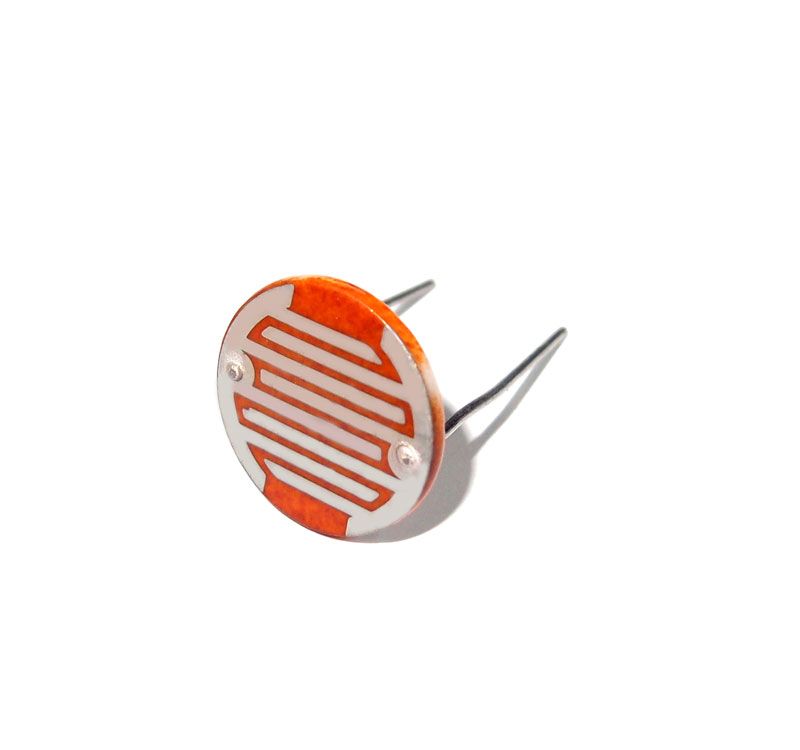
\includegraphics[scale=0.2]{sensor.jpg}\\
			
		\end{center}
	\end{figure}
	%------------------------------------------------
	%	Author(s)
	%------------------------------------------------
	
	\begin{minipage}{0.5\textwidth}
		\begin{flushleft}
			\large
			\textit{Lecturer: }\\
			 \textsc{Nguyen Tran Huu Nguyen} % Your name
		\end{flushleft}
	\end{minipage}
	~
	\begin{minipage}{0.4\textwidth}
		\begin{flushright}
			\large
			\textit{Course:}\\
			 \textsc{Electronic Devices and Circuit(Lab)} % Supervisor's name
		\end{flushright}
	\end{minipage}
	
	% If you don't want a supervisor, uncomment the two lines below and comment the code above
	%{\large\textit{Author}}\\
	%John \textsc{Smith} % Your name
	
	%------------------------------------------------
	%	Date
	%------------------------------------------------
	
	\vfill\vfill\vfill % Position the date 3/4 down the remaining page
	
	{\large May $8^{th}$, 2019} % Date, change the \today to a set date if you want to be precise
	
	%------------------------------------------------
	%	Logo
	%------------------------------------------------
	
	%\vfill\vfill
	%\includegraphics[width=0.2\textwidth]{placeholder.jpg}\\[1cm] % Include a department/university logo - this will require the graphicx package
	 
	%----------------------------------------------------------------------------------------
	
	\vfill % Push the date up 1/4 of the remaining page
	
\end{titlepage}

%----------------------------------------------------------------------------------------

\begin{center}
{\huge\bfseries GROUP MEMBERS}\\[1cm]

\end{center}
	\begin{minipage}{0.5\textwidth}
		\begin{flushleft}
			\large
			\textit{{\huge\bfseries NAME}\\[0.5cm]}
			 \textsc{{Ngo Qui Thu}\\[0.2cm]}
			 \textsc{{Nguyen Huu Gia Huy}\\[0.2cm]}
			 \textsc{{Tran Hoang Viet Long}\\[0.2cm]}
			 \textsc{{Truong Van Quang Dat}\\[0.2cm]}
			 \textsc{{Pham Le The Anh}\\[0.2cm]}
			 \textsc{{Vuong Le Huy}\\[0.2cm]}
		\end{flushleft}
	\end{minipage}
	~
	\begin{minipage}{0.5\textwidth}
		\begin{flushright}
			\large
			\textit{{\huge\bfseries ID}\\[0.5cm]}
			 \textsc{{1652595}\\[0.2cm]}
			 \textsc{{1652242}\\[0.2cm]}
			 \textsc{{1652350}\\[0.2cm]}
			 \textsc{{1652142}\\[0.2cm]}
			 \textsc{{1652026}\\[0.2cm]}
			 \textsc{{1652252}\\[0.2cm]}
		\end{flushright}
	\end{minipage}
\clearpage
%----------------------------------------------------------------------------------------

%{\huge\bfseries LIST OF CONTENTS:}\\[1cm]		

{\large\tableofcontents}


\maketitle

\section{Proceeding Steps}

\begin{figure}[ht]
		\begin{center}
			
			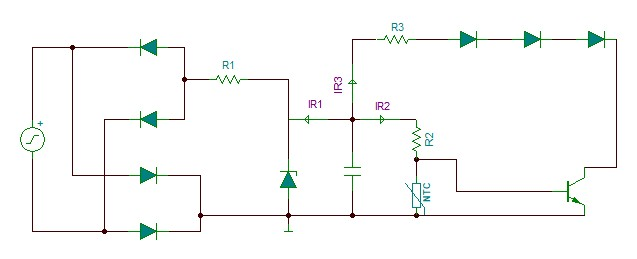
\includegraphics[scale=0.75]{PROJECT.JPG}\\[0,5cm]
			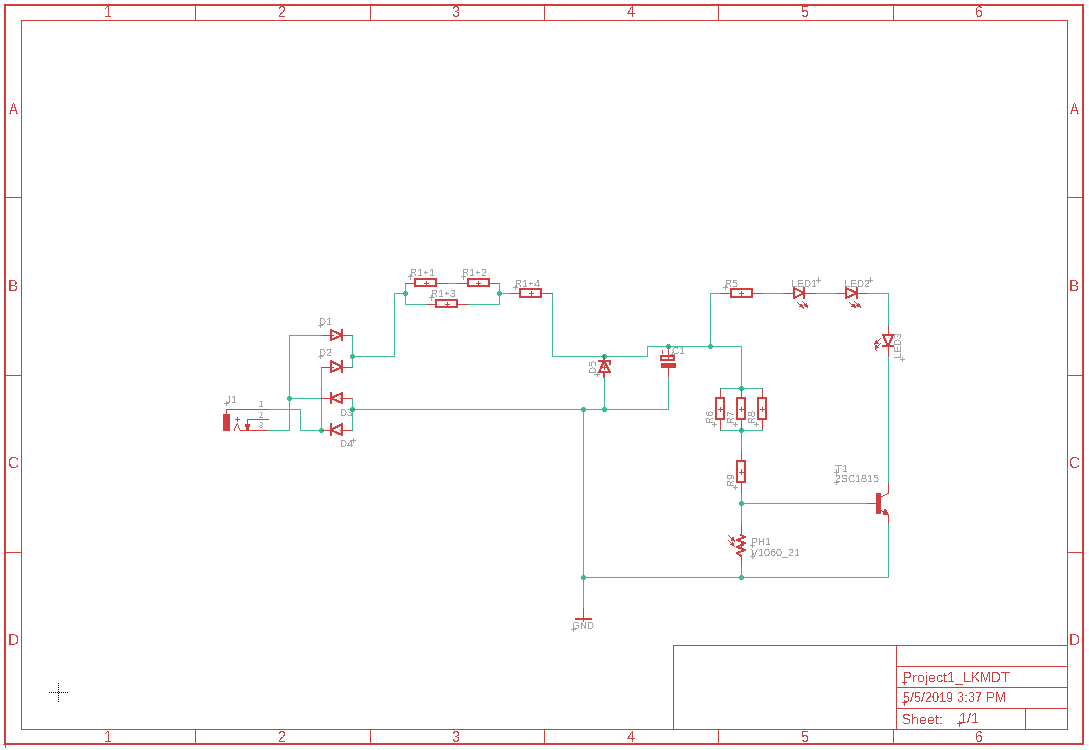
\includegraphics[scale=0.5]{sch.PNG}\\[0,5cm]
			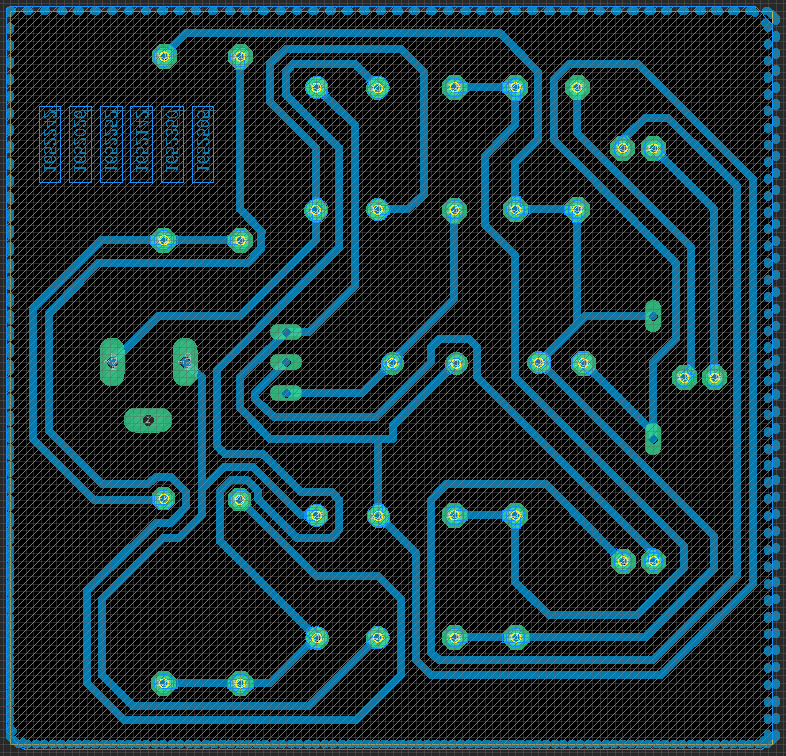
\includegraphics[scale=0.5]{Board.PNG}\\[0,5cm]
		\end{center}
\end{figure}
\begin{normalsize}
\tab $\blacktriangleright$ Circuit Analysis When System In Stand By State (No Sound Detected).
\begin{align*}
&V_{G1} = 0(V)
\end{align*}
Applying Kirchhoff's Voltage Law, this expression can be inferred:
\begin{align*}
&V_{R_{4,5}} = \frac{V_1 . R_5}{R_4 + R_5} = \frac{12x10}{10 + 10} (V)
\end{align*}
$\bullet$ Hence $V_2$ and $V_3$ share a common intput value of 6 volts, the output signal of\\Op-Amplifier is zero.  
\begin{align*}
&V_3 = V_2 = 6 (V)\\ 
\Longrightarrow &V_{2,3} = 0 (V)
\end{align*}
$\bullet$ Thus $V_{out}$ takes the same value with $V_{R_1}$ and $V_{R_2}$.
\begin{align*}
V_{out} = V_{R_1} = V_{R_2} = 6 (V)
\end{align*}
\tab $\blacktriangleright$ Circuit Analysis When System In Operation State (Clapping-Sound Is Recorded).
\begin{align*}
&V_{G1} \neq 0 (V)
\end{align*}
$\bullet$ If a sound is recorded. The microphone converts physical sound waves into electronic pulses. Eletronic signals run through wires to $C_1$ capacitor. $C_1$ is reposible for stablizing the pulses.\\
\\
This results in changes of $V_{mic}$:
\begin{align*}
&V_{mic} = 6 - V_{G1} (V)
\end{align*}
Electronically, a current would run through the circuit.
\begin{align*}
i = \frac{V_{mic}}{R_2} = \frac{V_{mic}}{1K(\Omega)} (A)
\end{align*}
Subsequently, $V_{out}$ suffers a voltage drop down.
\begin{align*}
&V_{out} = 6(V) - \frac{100K(\Omega).V_{G1}}{1K(\Omega)} (V)
\end{align*}
$\bullet $ Theoretically, Amplification at the output port $U_1$ is demonstrated in the expression\\below:
\begin{align*}
&U_1 = \frac{R3}{R_2} (V)
\end{align*}
Applying Nodal Analysis, $V_{ref}$ can be calculated by the following formular:
\begin{align*}
&V_{ref} = \frac{R_6}{R_6 + R_7}
\end{align*}
Similarly, through Nodal Analysis, $V_{rec}$ estimation is illustrated bellow:
\begin{align*}
&V_{Rec} = V_{out} - 0.7 (V)
\end{align*}
This results in $V_{rec} > V_{ref}$ which cause reversed polarity in the second amplifier.
\begin{align*}
&U_2 = 0(V)
\end{align*}
$\bullet $ Which means no electronic signal comes to Switch port.
\begin{align*}
&V_{sw} = 0(V)
\end{align*}
Meanwhile, the subsequent voltage differentitation at the two ends of LED1 makes it glow. \\
\\
$\bullet $ Hence $V_{sw}$ is connected to signal pin of IC 4017 counter so that $Y_1$ would be shifted to HIGH.\\
\\
In the meantime $Y_1$ triggers the collector pin of the C1815 NPN transitor C1815. At this point, a connection is established so that a current running though the coil is generated.\\
\\
Magnetic field of the coil attracts the switch conducing to connection between COM (Communication port) and NC (Normally closed port) which signals control of the\\ device.
%----------------------------------------------------------------------------------------
\clearpage
\section{Results Evaluation}
\tab $\triangleright$ Amplification: x100.\\
\tab $\triangleright$ Clapping range: 0.5(m).
\section{Application}
In spite of poor performance and improper functionality in noisy enviroment, the system performed flawlessly in quiet enviroment this could be attributed to the reason why clapping-switch system could be extensively used in controling home devices (lights, heating and air-conditioning systems, fans, etc). \\
\\
Nonetheless, more advanced, the system could be used as a cheap and economic theif dectecting system which functions as an ear listen to unidentified sound.\\
\\
However longer clapping range and more precise sound detection must be taken into account in order to make the system more user-friendly comercalizable.
\end{normalsize}
\end{document}
